\documentclass{scrartcl}
\usepackage{german}
\usepackage[T1]{fontenc}
\usepackage[utf8]{inputenc}
\usepackage[german]{babel}

% zusätzliche mathematische Symbole, AMS=American Mathematical Society
\usepackage{amssymb}

% fürs Einbinden von Graphiken
\usepackage{graphicx}

% für Namen etc. in Kopf- oder Fußzeile
\usepackage{fancyhdr}

% erlaubt benutzerdefinierte Kopfzeilen
\pagestyle{fancy}

% Definition der Kopfzeile
\lhead{
	\begin{tabular}{ll}
		Fisnik Zeqiri & 4306430 \\
		Felix  Karg   & 4342014
	\end{tabular}
}
\chead{}
\rhead{\today{}}
\lfoot{}
\cfoot{Seite \thepage}
\rfoot{}

\begin{document}
	\section*{Antworten zum �bungsblatt Nr. 3}

	\subsection*{Aufgabe 1}
	\begin{itemize}
	\item[a)] Funktionstabelle:

		\begin{table}[h]

			\begin{tabular}{c|c|c}
				Eingang & Ausgang & Realisierung \\
				\hline
				0,0 & 0 & AND \\
				0,0 & 1 & NAND \\
				0,1 & 0 & NOR \\
				0,1 & 1 & OR \\
				1,0 & 0 & NOR \\
				1,0 & 1 & OR \\
				1,1 & 0 & NAND \\
				1,1 & 1 & AND \\


			\end{tabular}
		\end{table}

    \newpage

	\item[b)] Gatter: \\
    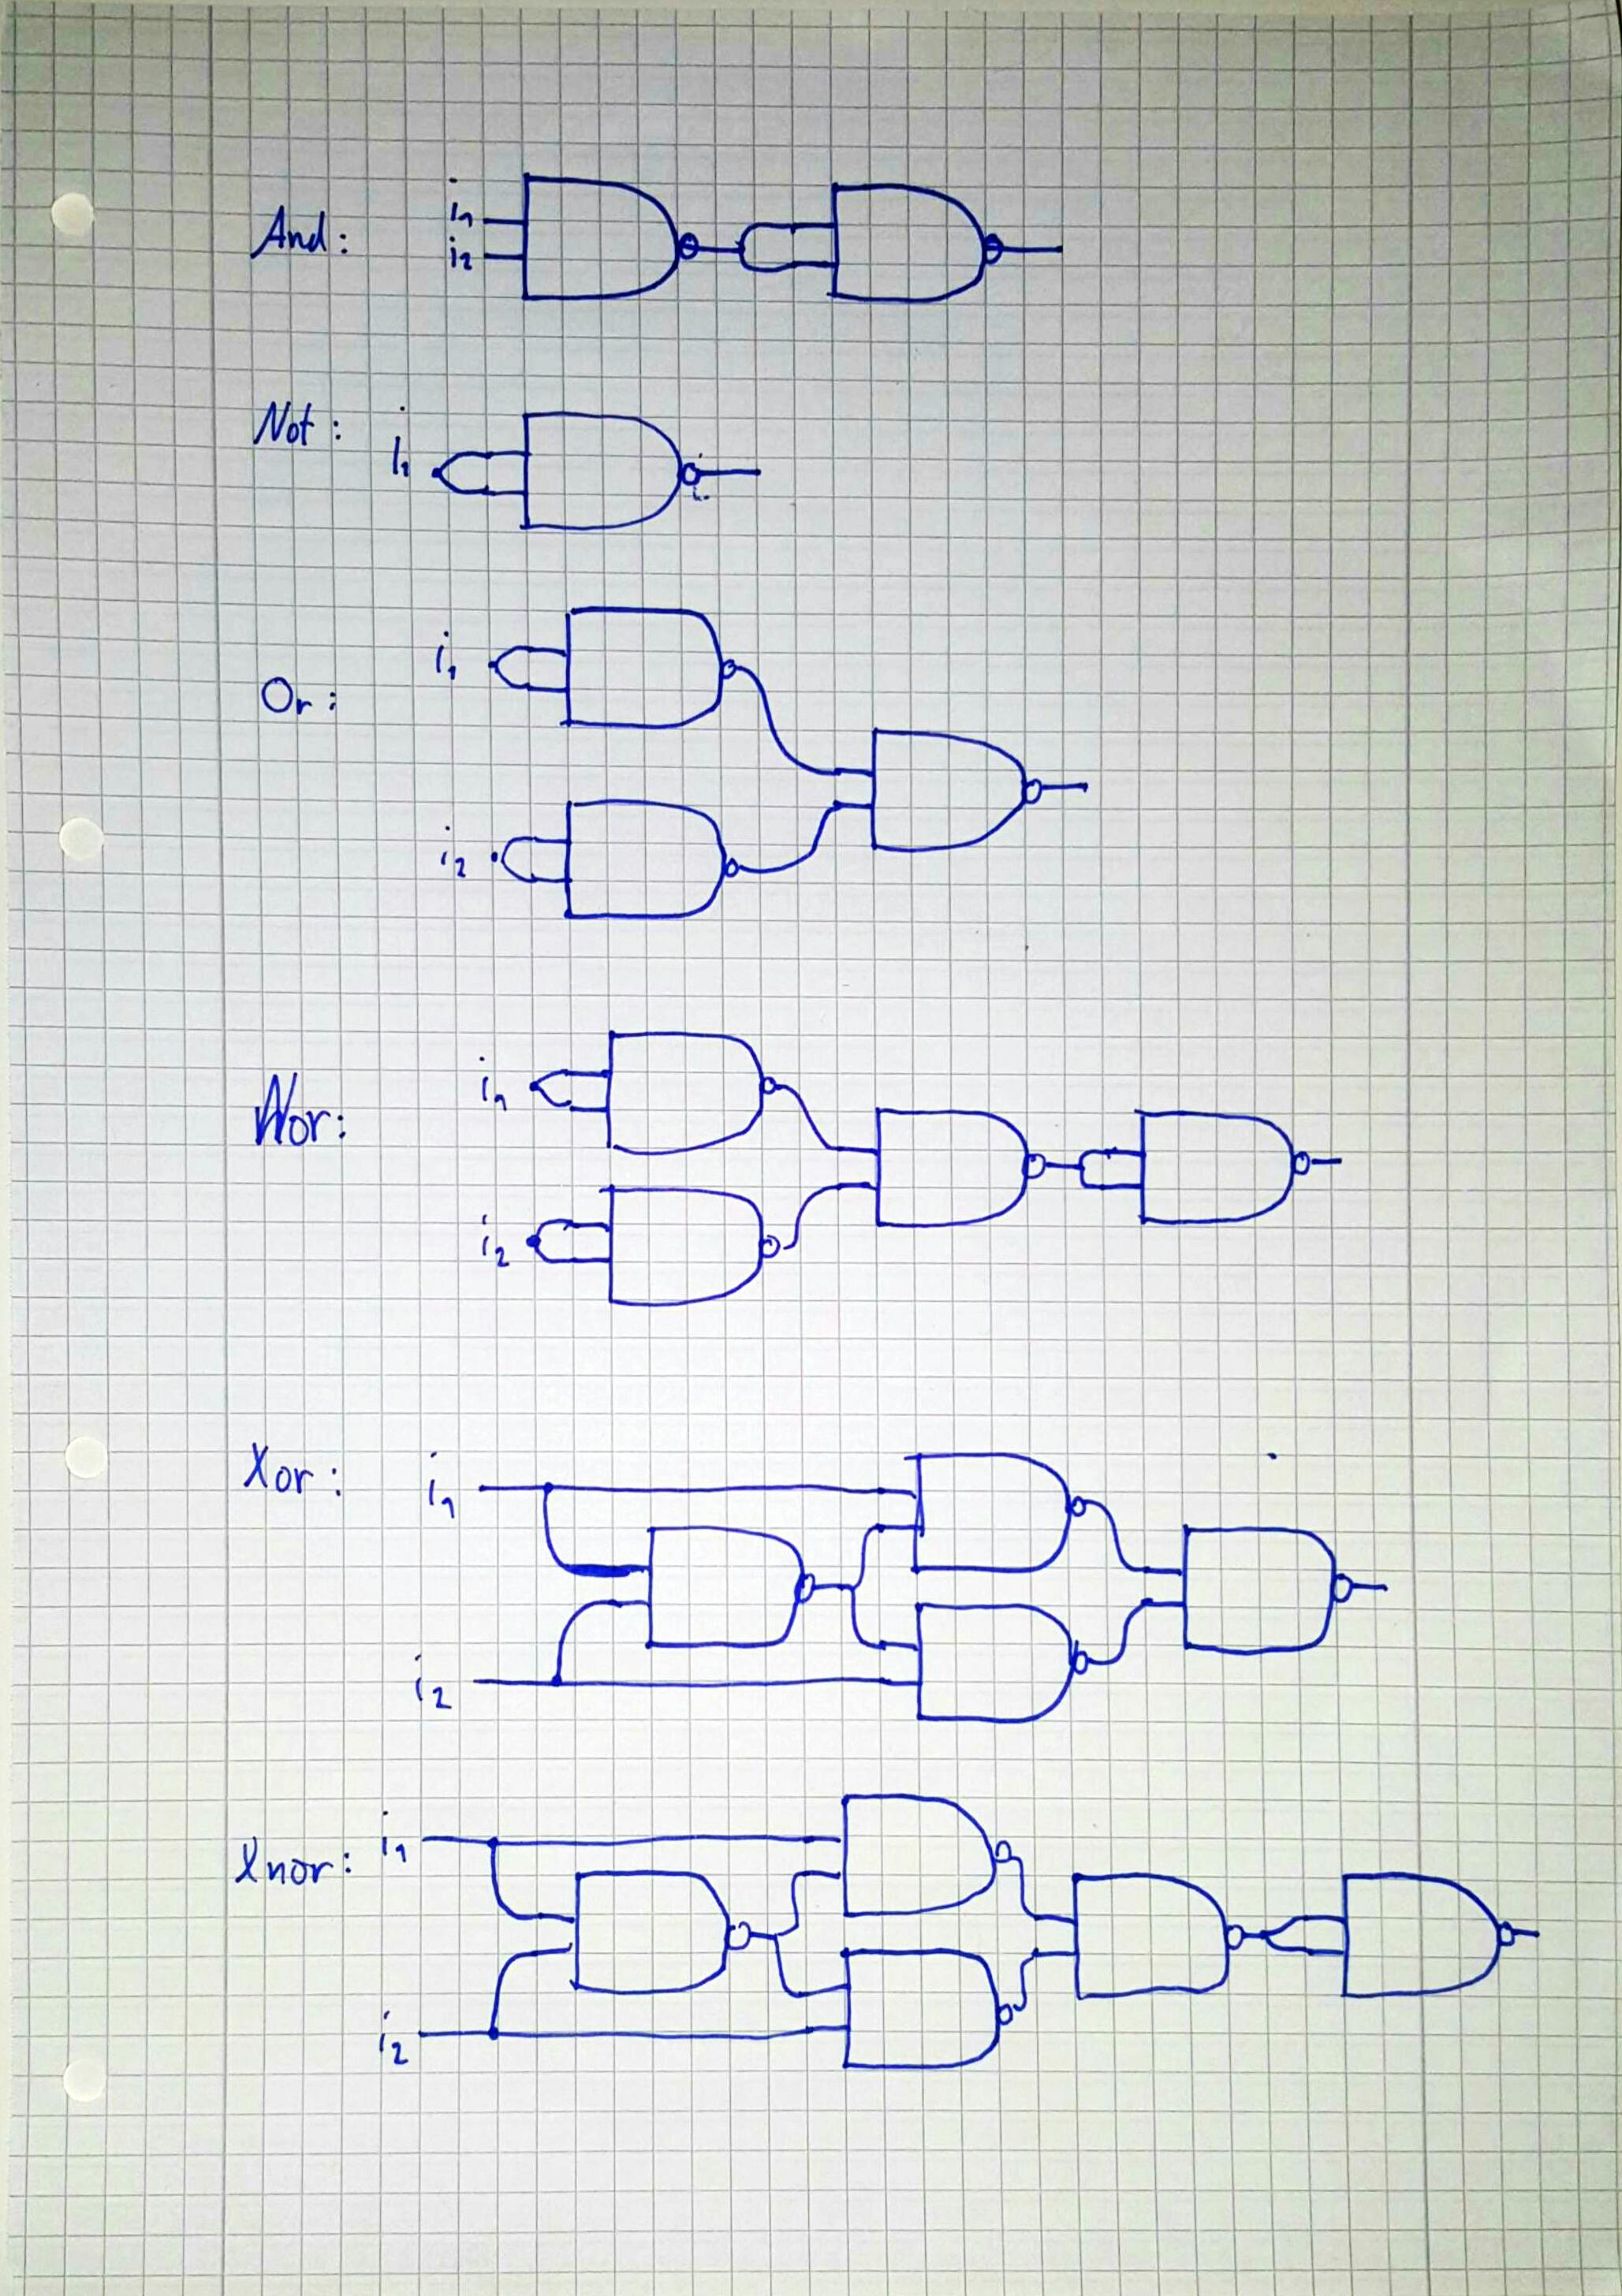
\includegraphics[width=14cm]{1b.jpg}



	\end{itemize}
	\subsection*{Aufgabe 2}
  sext\((y)\) ist die sign extension von y, d.h. egal in welcher darstellung y ist,
  wird y um die erwünschte (in diesem Fall 8) Anzahl bits erweitert, ohne den wert
  der eigentlichen Zahl zu verändern. Dadurch gilt war streng genommen
  $[$sext$(y)$]$ = $[$y$] nicht, da die sign extension immer $\geq$ Bits hat als die
  Ursprüngliche Zahl, allerdings muss der dergestellte Wert der Zahl gleich bleiben$^{[1]}$.
  \\ \\
  \verb![1] : https://en.wikipedia.org/wiki/Sign_extension!


%  Da [sext\((y)] = [00000000y_1...y_n] \) ist, und eine Positive Binäre Zahl egal in welcher
%  Darstellung (Binärbetrag mit Vorzeichen, Einer- bzw. Zweierkomplement) gleich dargestellt
%  wird, solange das erste bit 0 ist, ist eindeutig [sext\((y)] = [y] \). \hfill $\Box$
%         \\ \\
%
%         Zu beachten ist ist dass es nicht möglich ist, eine 24-bit große Zahl in einer 23-bit
%         großen Zahl mit Vorzeichen (-> 24bit) darzustellen, sollte das bit mit dem größten Wert
%         ($2^{24} = 16777216$) belegt sein, da die Zahl dann bereits größer ist als alles andere
%         was mit $2^{23}$ bits dargestellt werden kann.

	% Done ?


	\subsection*{Aufgabe 3}

	\begin{table}[h]

		\begin{tabular}{c|c|c|c}
			Zahl & Betrag mit Vorzeichen & Einerkomplement & Zweierkomplement \\
			\hline
			2342\textsubscript{10} & 0100100100110 & 0100100100110 & 0100100100110 \\

			-BFCD\textsubscript{16} & 11011111111001101 & 10100000000110010 & 10100000000110011 \\
			-10\textsubscript{16} & 110000 & 101111 & 10000 \\
			255\textsubscript{8} & 010101101 & 010101101 & 010101101 \\

		\end{tabular}
	\end{table}



	\subsection*{Aufgabe 4}
		\begin{itemize}

                \item[a)] Zwei Darstellungen f�r Null:\\
                Das Erste Bit d\textsubscript{n} gibt an, ob die Binärzahl komplementiert werden
                soll. Ist dies nicht der fall (d\textsubscript{n} = 0), ist die darstellung für
                die 0: \\
                \centerline{00. (beliebige anzahl an Nullen.)}\\
                ist d\textsubscript{n} = 1, so muss die Binärzahl komplementiert werden.
                Daher ist eine weitere Darstellunng für 0:\\
                \centerline{11. (beliebige anzahl an Einsen, da sie beim komplementieren zu Nullen
                werden.)}\\
                Also ergeben sich bei der Einer-Komplement-Darstellung genau zwei Darstellungen für
                die Null. \hfill $\Box$

                \item[b)]
                Gegeben ist dass die Zahl $$(\sum^{n-1}_{i=-k}2^i d_i) - d_n(2^n - 2^k)$$ ist,
                also die Summe von $-k$ bis $n-1$ über $2^id_i$. Die eindeutig Größte Zahl abhängig
                von diesen Parametern ist also die, bei der alle $d_i = 1$ sind und $d_n=0$. \\
                Da die in $n$ bits größte darstellbare Zahl $2^n -1$ ist, und die über die
                Nachkommerstellen ($k$) maximal darstellbare zahl von $0$ an $1$ annähert
                (Genauigkeit $2^{-k}$, also max: $1 - 2^{-k}$), ist die allgemein Größte
                darstellbare Zahl die Summe der beiden, also $2^n -1 + 1 - 2^{-k} = 2^n - 2^{-k}$.
                \\

                Die Kleinste darstellbare Zahl ist hingegen die bei der möglichst viele $d_i = 0$
                sind und $d_n = 1$, da dann die Summe null ergibt und $2^n - 2^{-k}$ abgezogen
                werden, ist die kleinste mit $n,k$ bits darstellbare Zahl (im Einserkomplement)
                $-(2^n - 2^{-k})$. \hfill $\Box$


		\item[c)]
                Wenn man alle bits $[d_n...d_0...d_{-k}]$ negiert ($b = 1 - b$) erhält man das
                absolute komplement zu dieser Zahl. Da das Einserkomplement symmetrisch ist,
                also jeweils die größte Darstellbare Zahl von der Restzahl subtrahiert wird,
                sowie die Restzahl auch quasi von der größte Darstellbaren
                Zahl subtrahiert wird (das komplement), ehrhält man nun direkt $-d$. \hfill $\Box$
		\end{itemize}

\end{document}
